\documentclass[12pt]{article}

%%%%%%%%%%%%%%%%%%%%%%%%%%%%%%%%%%%%%%%%%%%%%%%%%%%%%%%%%%%%%%%%%%%%%%%%%%%%%%%%
%                           Package preset for homework
%%%%%%%%%%%%%%%%%%%%%%%%%%%%%%%%%%%%%%%%%%%%%%%%%%%%%%%%%%%%%%%%%%%%%%%%%%%%%%%%
% Miscellaneous
\usepackage[margin=1in]{geometry}
\usepackage[utf8]{inputenc}
\usepackage{indentfirst}
\usepackage{blindtext}
\usepackage{graphicx}
\usepackage{xr-hyper}
\usepackage{hyperref}
\usepackage{enumitem}
\usepackage{color}
\usepackage{float}
% Math
\usepackage{latexsym}
\usepackage{amsfonts}
\usepackage{amssymb}
\usepackage{amsmath}
\usepackage{commath}
\usepackage{amsthm}
\usepackage{bbold}
\usepackage{bm}
% Physics
\usepackage{physics}
\usepackage{siunitx}
% Code typesetting
\usepackage{listings}
% Citation
\usepackage[authoryear]{natbib}
\usepackage{appendix}
\usepackage[capitalize]{cleveref}
% Title & name
\title{Homework}
\author{Tien Vo}
\date{\today}


%%%%%%%%%%%%%%%%%%%%%%%%%%%%%%%%%%%%%%%%%%%%%%%%%%%%%%%%%%%%%%%%%%%%%%%%%%%%%%%%
%                   User-defined commands and environments
%%%%%%%%%%%%%%%%%%%%%%%%%%%%%%%%%%%%%%%%%%%%%%%%%%%%%%%%%%%%%%%%%%%%%%%%%%%%%%%%
%%% Misc
\sisetup{load-configurations=abbreviations}
\newcommand{\due}[1]{\date{Due: #1}}
\newcommand{\hint}{\textit{Hint}}
\let\oldt\t
\renewcommand{\t}[1]{\text{#1}}

%%% Bold sets & abbrv
\newcommand{\N}{\mathbb{N}}
\newcommand{\Z}{\mathbb{Z}}
\newcommand{\R}{\mathbb{R}}
\newcommand{\Q}{\mathbb{Q}}
\let\oldP\P
\renewcommand{\P}{\mathbb{P}}
\newcommand{\LL}{\mathcal{L}}
\newcommand{\FF}{\mathcal{F}}
\newcommand{\HH}{\mathcal{H}}
\newcommand{\NN}{\mathcal{N}}
\newcommand{\ZZ}{\mathcal{Z}}
\newcommand{\RN}[1]{\textup{\uppercase\expandafter{\romannumeral#1}}}
\newcommand{\ua}{\uparrow}
\newcommand{\da}{\downarrow}

%%% Unit vectors
\newcommand{\xhat}{\vb{\hat{x}}}
\newcommand{\yhat}{\vb{\hat{y}}}
\newcommand{\zhat}{\vb{\hat{z}}}
\newcommand{\nhat}{\vb{\hat{n}}}
\newcommand{\rhat}{\vb{\hat{r}}}
\newcommand{\phihat}{\bm{\hat{\phi}}}
\newcommand{\thetahat}{\bm{\hat{\theta}}}

%%% Other math stuff
\providecommand{\units}[1]{\,\ensuremath{\mathrm{#1}}\xspace}
% Set new style for problem
\newtheoremstyle{problemstyle}  % <name>
        {10pt}                   % <space above>
        {10pt}                   % <space below>
        {\normalfont}           % <body font>
        {}                      % <indent amount}
        {\bfseries\itshape}     % <theorem head font>
        {\normalfont\bfseries:} % <punctuation after theorem head>
        {.5em}                  % <space after theorem head>
        {}                      % <theorem head spec (can be left empty, 
                                % meaning `normal')>

% Set problem environment
\theoremstyle{problemstyle}
\newtheorem{problemenv}{Problem}[section]
\newenvironment{problem}[1]{%
  \renewcommand\theproblemenv{#1}%
  \problemenv
}{\endproblemenv}
% Set lemma environment
\newenvironment{lemma}[2][Lemma]{\begin{trivlist}
\item[\hskip \labelsep {\bfseries #1}\hskip \labelsep {\bfseries #2.}]}{\end{trivlist}}
% Set solution environment
\newenvironment{solution}{
    \begin{proof}[Solution]$ $\par\nobreak\ignorespaces
}{\end{proof}}
\numberwithin{equation}{problemenv}

%%% Page format
\setlength{\parindent}{0.5cm}
\setlength{\oddsidemargin}{0in}
\setlength{\textwidth}{6.5in}
\setlength{\textheight}{8.8in}
\setlength{\topmargin}{0in}
\setlength{\headheight}{18pt}

%%% Code environments
\definecolor{dkgreen}{rgb}{0,0.6,0}
\definecolor{gray}{rgb}{0.5,0.5,0.5}
\definecolor{mauve}{rgb}{0.58,0,0.82}
\lstset{frame=tb,
  language=Python,
  aboveskip=3mm,
  belowskip=3mm,
  showstringspaces=false,
  columns=flexible,
  basicstyle={\small\ttfamily},
  numbers=none,
  numberstyle=\tiny\color{gray},
  keywordstyle=\color{blue},
  commentstyle=\color{dkgreen},
  stringstyle=\color{mauve},
  breaklines=true,
  breakatwhitespace=true,
  tabsize=4
}
\lstset{
  language=Mathematica,
  numbers=left,
  numberstyle=\tiny\color{gray},
  numbersep=5pt,
  breaklines=true,
  captionpos={t},
  frame={lines},
  rulecolor=\color{black},
  framerule=0.5pt,
  columns=flexible,
  tabsize=2
}


\title{Homework 6: Astr 5140 (Fall 2021)}

\begin{document}
\maketitle
%%%%%%%%%%%%%%%%%%%%%%%%%%%%%%%%%%%%%%%%%%%%%%%%%%%%%%%%%%%%%%%%%%%%%%%%%%%%%%%%
\begin{problem}{1}[Polarization drift]
In addition to $\vb{E}\times\vb{B}$ drift, there are of several high-order
plasma drifts. The polarization drift is one such drift that comes from a
time-varying electric field. Let $\vb{E}$ lie in the $y$ direction and $\vb{B}$
in the $z$ direction. We know that $v=\vb{E}\times\vb{B}/B^2$. In this problem
we want to derive $\vb{v}_p$ the polarization drift in the $y$ direction.

(a) Show that $\vb{v}_p=(m /qB^2)d\vb{E}_y /dt$. Treat $d\vb{E}_y /dt$ as a
constant. Hint: See Boyd \& Sanderson 2.12 (pg. 37).

(b) How does the polarization drift differ from the $\vb{E}\times\vb{B}$ drift?
Which has a faster polarization drift, ions or electrons? Why? What is the
current associated with the polarization drift?
\begin{solution}
(a) Given $\vb{E}=E\yhat$ and $\vb{B}=B\zhat$, the Lorentz force equation is
\begin{equation}
    m\dot{\vb{v}}=m\qty(\vb{E}+\vb{v}\times\vb{B})=q(E\yhat-v_xB\yhat+v_yB\xhat) 
    \Rightarrow
    \begin{cases}
        \dot{v}_x&=\Omega_cv_y\\
        \dot{v}_y&=qE/m-\Omega_cv_x
    \end{cases}
\end{equation}
where $\Omega_c=qB/m$. Then $v_y$ follows the differential equation
\begin{equation}
    \ddot{v}_y=\frac{q\dot{E}}{m}-\Omega_c^2v_y=
    -\Omega_c^2\qty(v_y-\frac{m}{qB^2}\dot{E})
\end{equation}
Let $\overline{v}_y=v_y-\frac{m}{qB^2}\dot{E}$, then since $\ddot{E}=0$,
$\overline{v}_y$ satisfies
\begin{equation}
    \ddot{\overline{v}}_y=-\Omega_c^2\overline{v}_y 
\end{equation}
A general solution to this is
\begin{equation}
    \overline{v}_y=v_\perp \sin(\Omega t+\delta)\Rightarrow
    v_y=v_\perp\sin\qty(\Omega t+\delta)+\frac{m}{qB^2}\frac{dE}{dt}
\end{equation}
where $v_\perp$ and $\delta$ depend on initial conditions. Thus, there is a
drift $v_p=(m/qB^2)\dot{E}_y$ in the $y$ direction beside the
$\vb{E}\times\vb{B}$ drift in the $x$ direction
\begin{equation}
    v_x=\frac{qE}{m\Omega_c}-\frac{\dot{v}_y}{\Omega_c}=-v_\perp\cos\qty(\Omega_ct+\delta)+\frac{E}{B}
\end{equation}

(b) While the $\vb{E}\times\vb{B}$ drift does not depend on the properties of
the charged particle (mass and charge), the polarization drift does. Since
$v_p\sim m$, ions drift faster than electrons. The current associated to this
drift is
\begin{equation}
    J_y=nqv_p=\frac{nm}{B^2}\frac{\partial E}{\partial t}
    =\frac{\rho}{B^2}\frac{\partial E}{\partial t}
\end{equation}
\end{solution}
\end{problem}
%%%%%%%%%%%%%%%%%%%%%%%%%%%%%%%%%%%%%%%%%%%%%%%%%%%%%%%%%%%%%%%%%%%%%%%%%%%%%%%% 
%%%%%%%%%%%%%%%%%%%%%%%%%%%%%%%%%%%%%%%%%%%%%%%%%%%%%%%%%%%%%%%%%%%%%%%%%%%%%%%%
\begin{problem}{2}[Inertial Alfvén wave]
In this problem, let $\vb{B}_0$ be in the $z$ direction and the motion,
$\vb{u}_1$ and $\vb{B}_1$ in the $x$ direction. An Alfvén wave that is nearly
perpendicular will have $k_y\gg k_z$ and will develop strong curents parallel to
$\vb{B}_0$. Assume that the parallel current can be represented by electron
motion
\begin{equation}\label{p2:1}
    \frac{\partial J_z}{\partial t}=\frac{ne^2}{m_e}E_z 
\end{equation}
while the perpendicular current is from the polarization drift
\begin{equation}\label{p2:2}
    J_y=\frac{\rho_0}{B_0^2}\frac{\partial E_y}{\partial t} 
\end{equation}
Derive the dispersion relation of the inertial Alfvén wave using the above
combined with Maxwell's equations. Express $\omega$ in terms of $\vb{k},V_A,$
and the electron skin depth ($\lambda_e=c /\omega_{pe})$. Hint: One does not
need the fluid equations once $\vb{J}$ is determined.
\begin{solution}
Given $\vb{B}_0=B_0\zhat,\vb{u}_1=u_1\xhat,\vb{B}_1=B_1\xhat,$ and
$\vb{k}=k_y\yhat+k_z\zhat$, we can Fourier transform Ampere's Law and write
\begin{equation}
    \curl{\vb{B}}=\mu_0\vb{J}
    \Rightarrow i(k_y\yhat+k_z\zhat)\times\qty(B_1\xhat)
    =iB_1\qty(-k_y\zhat+k_z\yhat)=\mu_0\vb{J}
\end{equation}
Thus,
\begin{equation}
    -ik_yB_1=\mu_0J_z=i\frac{\omega_{pe}^2}{\omega c^2}E_z\qquad\text{and}\qquad
    ik_zB_1=\mu_0J_y=-\frac{i\omega}{V_A^2}E_y
\end{equation}
where we have also Fourier transformed \eqref{p2:1} and \eqref{p2:2}. Similarly,
from Faraday's Law,
\begin{equation}
    (k_yE_z-k_zE_y)=-\frac{\omega
    c^2k_y^2}{\omega_{pe}^2}B_1+\frac{k_z^2V_A^2}{\omega}B_1=\omega B_1
    \Rightarrow -k_y^2\lambda_e^2+\frac{k_z^2V_A^2}{\omega^2}=1
\end{equation}
Rewriting, we get the dispersion relation
\begin{equation}
    \omega^2=\frac{k_z^2V_A^2}{1+k_y^2\lambda_e^2} 
\end{equation}
\end{solution}
\end{problem}
%%%%%%%%%%%%%%%%%%%%%%%%%%%%%%%%%%%%%%%%%%%%%%%%%%%%%%%%%%%%%%%%%%%%%%%%%%%%%%%%
%%%%%%%%%%%%%%%%%%%%%%%%%%%%%%%%%%%%%%%%%%%%%%%%%%%%%%%%%%%%%%%%%%%%%%%%%%%%%%%%
\begin{problem}{3}[High Mach shocks]
The universe is full of plasmas in motion that encounter obstacles such as
stellar and planetary magnetospheres or other moving plasmas. If the motions
exceed the Alfvén or sound speed, a shock can form. One possibility is that the
flow perpendicular to the magnetic field. Mathematically, we model the shock
with time-stationary ``jump'' conditions in a frame where the shock is
stationary. 

(a) Write down the Rankine-Hugoniot jump conditions applicable for a
perpendicular shock.

(b)Using the compression ratio $r=\rho_2/\rho_1$, derive an expression for $P_2$
in terms of $r,\rho_1,u_1$, and $B_1$ by combining equations for continuity,
magnetic field, and force.

(c) Repeat the above calculation using the energy equation instead of the force
equation, that is, derive another expression for $P_2$ in terms of
$r,\rho_1,u_1$, and $B_1$ based on the energy equation.

(d) With a good bit of algebra, one could solve for the compression ratio $r$ in
terms of $P_1,\rho_1,u_1$, and $B_1$. Instead, let's introduce two new
quantities. Write down expressions for the upstream Mach numbers in terms of
$P_1,\rho_1,u_1$, and $B_1$.

(e) Derive approximations for expressions (a) and (b) assuming that $M_A\gg1$
and $M_s\gg1$.

(f) Demonstrate that, if $\gamma=5/3$, the compression ratio for a high-Mach
shock is 4.
\begin{solution}
(a) The jump conditions are as follows
\begin{subequations}
    \begin{align}
        \rho_1u_1&=\rho_2u_2\label{p3a:continuity}\\
        u_1B_1&=u_2B_2\label{p3a:maxwell}\\
        P_1+\rho_1u_1^2+\frac{B_1^2}{2\mu_0}&=P_2+\rho_2u_2^2+\frac{B_2^2}{2\mu_0}\label{p3a:force}\\
        u_1\qty(\frac12\rho_1u_1^2+\frac{\gamma}{\gamma-1}P_1+\frac{B_1^2}{\mu_0})&=u_2\qty(\frac12\rho_2u_2^2+\frac{\gamma}{\gamma-1}P_2+\frac{B_2^2}{\mu_0})\label{p3a:energy}
    \end{align} 
\end{subequations}

(b) From \eqref{p3a:continuity} and \eqref{p3a:maxwell}, the compression ratio
is
\begin{equation}
    r=\frac{\rho_2}{\rho_1}=\frac{u_1}{u_2}=\frac{B_2}{B_1} 
\end{equation}
Then from the force equation \eqref{p3a:force},
\begin{align}\label{p3b:P}
    P_2&=P_1+\rho_1u_1^2+\frac{B_1^2}{2\mu_0}-\rho_2u_2^2-\frac{B_2^2}{2\mu_0}\notag\\
       &=P_1+\rho_1u_1^2\qty(1-\frac{\rho_2}{\rho_1}\frac{u_2^2}{u_1^2})
   +\frac{B_1^2}{2\mu_0}\qty(1-\frac{B_2^2}{B_1}^2)\notag\\
       &=P_1+\rho_1u_1^2\qty(1-\frac1r)+\frac{B_1^2}{2\mu_0}\qty(1-r^2)
\end{align}

(c) Similary, from \eqref{p3a:energy},
\begin{align}\label{p3c:P}
    P_2&=\frac{\gamma-1}{\gamma}\qty[\frac{u_1}{u_2}\qty(\frac12\rho_1u_1^2+\frac{\gamma}{\gamma-1}P_1+\frac{B_1^2}{\mu_0})-\frac12\rho_2u_2^2-\frac{B_2^2}{\mu_0}]\notag\\
       &=P_1+\frac{\gamma-1}{\gamma}\qty[
       \frac12\rho_1u_1^2\qty(\frac{u_1}{u_2}-\frac{\rho_2}{\rho_1}\frac{u_2^2}{u_1^2})+\frac{B_1^2}{\mu_0}\qty(\frac{u_1}{u_2}-\frac{B_2^2}{B_1^2})
       ]\notag\\
       &=P_1+\frac{\gamma-1}{\gamma}\qty[
            \frac12\rho_1u_1^2\qty(r-\frac1r)+\frac{B_1^2}{\mu_0}\qty(r-r^2)
       ]
\end{align}

(d) By definition,
\begin{equation}
    M_A^2+\frac{u_1^2}{V_A^2}=\frac{(1/2)\rho_1u_1^2}{B_1^2/2\mu_0}
    \qquad\text{and}\qquad
    M_s^2=\frac{u_1^2}{\gamma T_1/m}
    =\frac{1}{\gamma}\frac{\rho_1^2u_1^2}{P_1}
\end{equation}

(e) At high $M_A$ and $M_s$, $\rho_1u_1^2\gg B_1^2/2\mu_0$ and $\rho_1 u_1^2\gg
P_1$. Thus, from \eqref{p3b:P} and \eqref{p3c:P},
\begin{equation}\label{p3e}
    P_2\approx\rho_1u_1^2\qty(1-\frac1r)\approx\frac{\gamma-1}{\gamma}\frac12\rho_1u_1^2(r-\frac1r)\Rightarrow\frac{\gamma-1}{\gamma}=2\frac{1-1/r}{r-1/r}\Leftrightarrow
    \frac{\gamma-1}{2\gamma}\qty(r^2-1)=r-1
\end{equation}

(f) When $\gamma=5/3$, \eqref{p3e} becomes
\begin{equation}
    \frac15r^2-r+\frac45=0\Rightarrow r=1\text{ or }r=4
\end{equation}
The first solution is trivial. So for a high Mach shock, $r=4$.
\end{solution}
\end{problem}
%%%%%%%%%%%%%%%%%%%%%%%%%%%%%%%%%%%%%%%%%%%%%%%%%%%%%%%%%%%%%%%%%%%%%%%%%%%%%%%%
%%%%%%%%%%%%%%%%%%%%%%%%%%%%%%%%%%%%%%%%%%%%%%%%%%%%%%%%%%%%%%%%%%%%%%%%%%%%%%%
\begin{problem}{4}[Harris Current Sheet - Review]
Assume a sheet of current in which $J$ flows in the $y$ direction. There is no
external magnetic field. Let $P=0$ and $B_z=\mp B_0$ at $x=\pm\infty$. One way
to find a physical solution is to set $\vb{J}$ to be proportional to $P$. Derive
a solution for $\vb{B},\vb{J}$, and $P$ by assuming $J_y=2P/(LB_0)$. $L$ is a
characteristic length. Plot $B_z,P$, and $J_y$ as a function of $x$.
\begin{solution}
The force equation is
\begin{equation}\label{p4:P}
    0=-\grad P-\grad\qty(\frac{B^2}{2\mu_0}) 
    \Rightarrow P+\frac{B^2}{2\mu_0}=\frac{B_0^2}{2\mu_0}
\end{equation}
where the RHS is given from boundary conditions. From Faraday's Law,
\begin{equation}
    -\frac{\partial B_z}{\partial
    x}=\mu_0J=\frac{B_0^2-B^2}{LB_0} 
\end{equation}
We can solve this differential equation by separation of variables
\begin{equation}
    \int\frac{dx}{L}=-B_0\int\frac{dB_z}{B_0^2-B^2}\Rightarrow\frac{x}{L}=-\tanh^{-1}\qty(\frac{B}{B_0})
\end{equation}
Then the magnetic field is
\begin{equation}
    B=-B_0\tanh(\frac{x}{L}) 
\end{equation}
Note that $B\to\mp B_0$ as $x\to\pm\infty$. This would create a current in the
$+y$ direction through the right hand rule. From \eqref{p4:P},
\begin{equation}
    P=\frac1{2\mu_0}(B_0^2-B^2)=\frac{B_0^2}{2\mu_0}\sech^2\qty(\frac{x}{L}) 
\end{equation}
and by assumption,
\begin{equation}
    J=\frac{B_0}{\mu_0L}\sech^2\qty(\frac{x}{L}) 
\end{equation}
Their plots are as below.
\begin{center}
    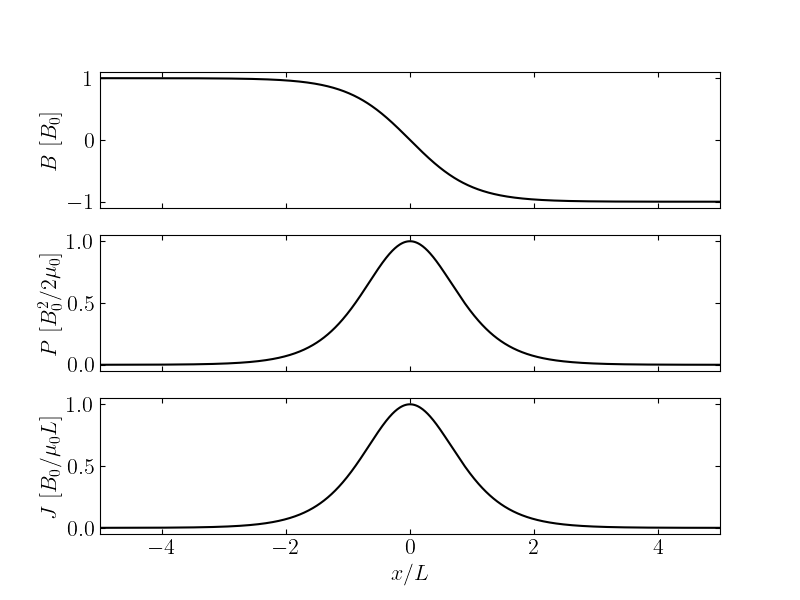
\includegraphics[width=1\textwidth]{p4.png} 
\end{center}
\end{solution}
\end{problem}
%%%%%%%%%%%%%%%%%%%%%%%%%%%%%%%%%%%%%%%%%%%%%%%%%%%%%%%%%%%%%%%%%%%%%%%%%%%%%%%
\end{document}
